% ============================================================
%  Paper VII  --  Referee version
%  Dyadic Cancellation for PSWF Galerkin Operators
%  Status: unconditional (Phase Non-Degeneracy resolved in
%          companion note phase_nondeg_lemma.tex)
% ============================================================
\documentclass[12pt]{amsart}

% --- packages ---
\usepackage{amsmath,amssymb,amsthm}
\usepackage{mathtools}
\usepackage{hyperref}
\usepackage{tikz}
\usetikzlibrary{arrows.meta, positioning}

% --- theorem environments ---
\newtheorem{theorem}{Theorem}[section]
\newtheorem{proposition}[theorem]{Proposition}
\newtheorem{corollary}[theorem]{Corollary}
\newtheorem{lemma}[theorem]{Lemma}
\theoremstyle{definition}
\newtheorem{assumption}[theorem]{Assumption}
\newtheorem{conjecture}[theorem]{Conjecture}
\theoremstyle{remark}
\newtheorem{remark}[theorem]{Remark}

% --- macros ---
\newcommand{\norm}[1]{\lVert#1\rVert}
\newcommand{\abs}[1]{\lvert#1\rvert}
\newcommand{\Bm}{\mathcal{B}_m}
\newcommand{\Bprime}{B^{\prime}}
\newcommand{\lam}[1]{\lambda_{#1}^{(c)}}

% ============================================================
\begin{document}
% ============================================================

\title[Dyadic Cancellation for PSWF Galerkin Operators]
      {Dyadic Cancellation for Oscillatory Kernels\\and
       Reduction of the PSWF Galerkin Contraction Problem}

\author{[Author]}
\date{\today}
\maketitle

% ------------------------------------------------------------
% PATCH 2: Abstract upgraded to unconditional
% ------------------------------------------------------------
\begin{abstract}
We establish unconditional spectral stability results for
discrete prolate spheroidal wave functions in the high-frequency
regime.
We prove an abstract dyadic cancellation theorem
(Theorem~\ref{thm:dyadic_cancellation}) for oscillatory kernels
with slowly varying amplitudes and reduce the contraction problem
for the PSWF Galerkin iteration to the verification of a global
amplitude bound (Assumption~\ref{ass:Bstrong}) and a local
amplitude regularity condition (Conjecture~\ref{conj:amplitude}).

All previously conditional assumptions in the phase structure
are now resolved:
the phase non-degeneracy condition required by
Theorem~\ref{thm:dyadic_cancellation} is proved unconditionally
in the companion note \cite{PhaseNondeg}
via a microlocal Airy--WKB stability lemma,
yielding $\alpha^{(c)} = \pi/2 + O(c^{-1/3})$
uniformly in the Galerkin regime $k \le N = \lfloor Ac^{1/3}\rfloor$.
As a consequence, the main structural decomposition is
independent of any phase non-degeneracy assumptions:
H1 holds unconditionally, and
Theorem~\ref{thm:dyadic_cancellation} applies unconditionally
for all $c \ge c_0(A)$.

The remaining open problems are precisely isolated:
the B-strong amplitude bound and amplitude regularity
on dyadic blocks (see Section~\ref{sec:open}).
\end{abstract}

% ============================================================
\section{Introduction}
\label{sec:intro}
% ============================================================

In Paper~VI \cite{paperVI} we established a No-go theorem
for the PSWF Galerkin operator:\,purely Schur-class
(non-oscillatory) decay estimates are insufficient to
establish contraction of the iteration map $\mathcal{T}_c^{(N)}$.
The central lesson of that paper is the factorisation
\[
  \text{Decay} \;\neq\; \text{Cancellation}.
\]
Cancellation is a separate structural property, and
classical Schur-class methods end precisely at this point.

The present paper takes the next step.
We show that cancellation is governed by an abstract mechanism
operating at the level of \emph{dyadic oscillatory sums},
independent of the PSWF model.
The mechanism requires three structural hypotheses
(H1)--(H3) on the kernel matrix and, when verified,
yields a norm bound that implies contraction and,
ultimately, a unique fixed point establishing Assumption~A.

Since the first version of this paper,
the phase non-degeneracy condition (H1, non-degeneracy part)
has been resolved unconditionally in \cite{PhaseNondeg}.
The structure of the proof is now:
\begin{itemize}
  \item H1 (phase): unconditional (see Proposition~\ref{prop:PSWF_hypotheses}(a))
  \item H2 (amplitude regularity): conditional on Conjecture~\ref{conj:amplitude}
  \item H3 (amplitude bound): conditional on Assumption~\ref{ass:Bstrong}
\end{itemize}

\medskip\noindent
\textbf{Informal statement of the main result.}
Let $T$ be a matrix with off-diagonal entries decaying
like $|i-j|^{-1}$, a non-degenerate oscillatory phase,
and slowly varying amplitude.
Then the row sums of $T$ are $O(1)$, controlled
uniformly in the matrix size.

\medskip\noindent
\textbf{Structure of the paper.}
Section~\ref{sec:cancellation} states and proves
Theorem~\ref{thm:dyadic_cancellation} (Abstract Cancellation).
Section~\ref{sec:PSWF} verifies the hypotheses for the PSWF
Galerkin operator (Proposition~\ref{prop:PSWF_hypotheses}).
Section~\ref{sec:closure} collects the implication chain
in Corollary~\ref{cor:closure}.
Section~\ref{sec:open} states the remaining open problems.
Appendix~\ref{sec:appendix} contains the complete proof
of Theorem~\ref{thm:dyadic_cancellation}.

% ============================================================
\section{Abstract Cancellation for Oscillatory Kernels}
\label{sec:cancellation}
% ============================================================

\subsection{Setup and hypotheses}

Let $N\in\mathbb{N}$ and let $T=(T_{ij})_{1\leq i,j\leq N}$
be a matrix of the form
\[
  T_{ij} = \frac{A_{ij}}{\abs{i-j}}\,e^{i\Phi_{ij}},
  \qquad i\neq j,\qquad T_{ii}=0.
\]
For fixed $i$, define dyadic blocks
\[
  \mathcal{B}_m(i):=\{j:\;2^m\leq\abs{i-j}<2^{m+1}\},
  \qquad m=0,\dots,M,\quad M=\lfloor\log_2 N\rfloor.
\]

We impose three hypotheses.

\medskip\noindent
\textbf{(H1) Non-degenerate phase direction.}
There exists $\alpha\in(0,2\pi)$,
$\alpha\not\equiv 0,\pi\pmod{2\pi}$, such that
\[
  \Phi_{ij} = \alpha(i-j) + \varepsilon_{ij},
\]
where the block-level phase errors
$\epsilon_m^{(N)} := \sup_{j\in\mathcal{B}_m(i)}\abs{\varepsilon_{ij}}$
satisfy
\[
  \sum_{m=0}^{\lfloor\log_2 N\rfloor} \epsilon_m^{(N)}
  = o(1)
  \qquad\text{as } N\to\infty.
\]

\medskip\noindent
\textbf{(H2) Blockwise amplitude regularity.}
There exists a sequence $\delta_m\to 0$ such that
for all $j,j+1\in\Bm(i)$,
\[
  \abs{A_{ij}-A_{i,j+1}}
  \leq \delta_m\,\frac{A_{ij}}{2^m}.
\]

\medskip\noindent
\textbf{(H3) Uniform amplitude bound.}
\[
  0 \leq A_{ij} \leq C
  \quad\text{for all } i\neq j,
\]
with $C$ independent of $N$.

\begin{remark}[Interpretation of the hypotheses]
Condition (H2) expresses that $A_{ij}$ varies on the
natural spectral scale $2^m$ at a relative rate $o(1)$
only, which is exactly the regime required for blockwise
Abel summation in the proof below.
The conclusion is stable under replacing $\abs{i-j}^{-1}$
by any kernel $K(i-j)$ satisfying $K(n)\sim\abs{n}^{-1}$
on dyadic blocks.
The critical feature is the borderline non-summability
$\sum_n n^{-1} = \infty$,
which is the mechanism forcing cancellation rather than
absolute convergence.

\medskip\noindent
The summability condition $\sum_m\epsilon_m^{(N)}=o(1)$
in (H1) is the minimal quantitative requirement: it controls
the \emph{total accumulated phase deviation} across all
dyadic scales, which is the precise quantity appearing
in Step~6 of the proof.
\end{remark}

\begin{remark}[Scaling and operator norm]
\label{rem:scaling}
In the PSWF application, the matrix $T_{ij}$ represents the
rescaled kernel $P_{ij}\,c^{1/2}$.
The bound $O(1)$ in Theorem~\ref{thm:dyadic_cancellation}
therefore corresponds to $O(c^{-1/2})$ for the original
operator $P_{ij}$.
The additional $\log c$ factor arises from the number of
dyadic blocks $M \sim \log N \sim \tfrac{1}{3}\log c$;
this logarithm is not accidental, but is precisely the
price of operating in the critical $1/n$ regime where
cancellation acts blockwise rather than absolutely.
In particular, this bound controls the operator norm of the
linearisation via the $\ell^\infty$--Schur estimate used
in Paper~VI~\cite{paperVI}:
\[
  \norm{D\mathcal{T}_c^{(N)}}_{\ell^\infty\to\ell^\infty}
  \leq
  \sup_i \sum_{j\neq i} \abs{P_{ij}}
  \leq C\,c^{-1/2}\log c.
\]
\end{remark}

\subsection{Main theorem}

\begin{theorem}[Dyadic oscillatory cancellation]
\label{thm:dyadic_cancellation}
Under hypotheses \textup{(H1)--(H3)}, for each $i$,
\[
  S_m(i):=\sum_{j\in\Bm(i)} T_{ij}
  = O\!\left(\frac{1}{2^m}\right)
\]
uniformly in $i$, with constants depending only on $\alpha$
and $C$.
Consequently,
\[
  \sup_{1\leq i\leq N}\sum_{j\neq i}\abs{T_{ij}} = O(1).
\]
\end{theorem}

\begin{proof}[Proof idea]
The proof proceeds by Abel summation on each dyadic block
$\Bm(i)$, using the Dirichlet kernel bound
$\abs{\sum_{k=J_1}^j e^{i\alpha(i-k)}} \leq C_\alpha$
(valid since $\alpha\not\equiv 0,\pi$)
together with the total-variation estimate
$\mathrm{TV}(A_{i\cdot};\Bm) = O(\delta_m)$
from (H2) and the uniform bound (H3).
Each block contributes $O(2^{-m})$, and
summing over $M+1 = O(\log N)$ blocks gives $O(1)$.
The complete proof with explicit constants is given
in Appendix~\ref{sec:appendix}.
\end{proof}

% ============================================================
\section{Verification for the PSWF Galerkin Operator}
\label{sec:PSWF}
% ============================================================

\begin{assumption}[B-strong: phase-sensitive coupling]
\label{ass:Bstrong}
For all $k\neq l$, $k,l\leq N = \lfloor Ac^{1/3}\rfloor$:
\[
  P_{kl} := c\cdot
  \frac{\abs{\lam{l}-\lam{k}}}{(1-\lam{k})(1-\lam{l})}
  \leq C_2\,c^{1/2}.
\]
\end{assumption}

\begin{assumption}[$B'$]
\label{ass:Bprime}
\[
  \sup_{i\leq N}\sum_{j\neq i}P_{ij}\cdot\abs{I_{ij}}
  \leq C\,c^{-1/2}\log c,
\]
where $I_{ij}:=\int_{-1}^1\arccos(s)\,\psi_i^{(c)}(s)\psi_j^{(c)}(s)\,ds$.
Not implied by Assumption~\ref{ass:Bstrong};
requires signed oscillatory cancellation.
\end{assumption}

\begin{conjecture}[Amplitude regularity on dyadic blocks
  {\normalfont(Conjecture~6.2 of \cite{paperVI})}]
\label{conj:amplitude}
For the amplitudes $A_{ij}:=P_{ij}\cdot c^{1/2}$ (normalised),
on each dyadic block
$\mathcal{B}_m(i)=\{j:2^m\leq\abs{i-j}<2^{m+1}\}$:
\[
  \abs{A_{ij}-A_{i,j+1}}
  = o\!\left(\frac{A_{ij}}{2^m}\right)
  \quad\text{uniformly in }i,j\in\mathcal{B}_m(i),\;
  m\leq M,
\]
with constants independent of $c$.
\end{conjecture}

\begin{proposition}[PSWF satisfies hypotheses of
  Theorem~\ref{thm:dyadic_cancellation}]
\label{prop:PSWF_hypotheses}
Let $k,l \leq N = \lfloor Ac^{1/3} \rfloor$ and set
\[
  T_{ij} = \frac{A_{ij}}{\abs{i-j}}\,e^{i\Phi_{ij}},
  \qquad
  A_{ij} := P_{ij} \cdot c^{1/2},
  \quad
  \Phi_{ij} := \Theta_i^{(c)} - \Theta_j^{(c)}.
\]

\medskip\noindent
\textbf{(a) H1 holds unconditionally.}
By Widom eigenvalue asymptotics,
\[
  \Phi_{ij} = \alpha^{(c)}(i-j) + O(\abs{i-j}^2/c)
\]
with $\alpha^{(c)} \in (0,\pi)$ given by Widom's formula.
The phase error satisfies $\abs{\varepsilon_{ij}}
\leq C\,\abs{i-j}^2/c$ pointwise, so
$\epsilon_m^{(N)} \leq C\,2^{2m}/c$.
Using $2^m \leq N \sim c^{1/3}$,
\[
  \frac{2^{2m}}{c} \leq c^{-1/3},
\]
and hence
\[
  \sum_{m=0}^{M} \epsilon_m^{(N)}
  \leq C\,c^{-1/3}(M+1)
  \leq C\,c^{-1/3}\log c \to 0.
\]
The summability condition of \textup{(H1)} is satisfied
unconditionally.

% ---------------------------------------------------------
% PATCH 1: H1 Non-Degeneracy -- 3-line version
% ---------------------------------------------------------
\medskip\noindent
\textbf{H1 Non-Degeneracy (unconditional).}

\begin{proposition}[H1 Non-Degeneracy]
\label{prop:H1_nondeg}
The phase non-degeneracy condition
\[
  \mathrm{dist}\bigl(\alpha^{(c)},\,\{0,\pi\}\bigr)
  \ge \frac{\pi}{4}
\]
holds uniformly for all $c \ge c_0(A)$
and all $k \le N = \lfloor Ac^{1/3}\rfloor$.
\end{proposition}

\begin{proof}
This follows directly from Corollary~1 of \cite{PhaseNondeg},
which establishes
$\alpha^{(c)} = \pi/2 + O(c^{-1/3})$
uniformly in the Galerkin regime via a microlocal
Airy--WKB stability argument.
\end{proof}

Combining the summability part and Proposition~\ref{prop:H1_nondeg},
hypothesis \textup{(H1)} holds in full, unconditionally.

\medskip\noindent
\textbf{(b) H2 holds under Conjecture~\ref{conj:amplitude}.}
The amplitude regularity condition
\[
  \abs{A_{ij}-A_{i,j+1}} \leq \delta_m\,\frac{A_{ij}}{2^m},
  \qquad \delta_m \to 0 \text{ uniformly in } c,
\]
is precisely the content of Conjecture~\ref{conj:amplitude}.

\medskip\noindent
\textbf{(c) H3 holds under Assumption~\ref{ass:Bstrong}.}
The normalisation $A_{ij} = P_{ij} \cdot c^{1/2}$ is chosen
so that $A_{ij} = O(1)$ is equivalent to
Assumption~\ref{ass:Bstrong}; explicitly,
$A_{ij} \leq C_2$ uniformly for all $i \neq j$,
$i,j\leq N$.
\end{proposition}

\begin{remark}[H1 is now closed]
\label{rem:H1_closed}
With Proposition~\ref{prop:H1_nondeg},
Conjecture~6.1 of \cite{paperVI} is proved.
The status of all three hypotheses:
\begin{itemize}
  \item H1 (phase non-degeneracy): \textbf{proved unconditionally}
        \cite{PhaseNondeg}
  \item H2 (amplitude regularity): open (Conjecture~\ref{conj:amplitude})
  \item H3 (amplitude bound): open (Assumption~\ref{ass:Bstrong})
\end{itemize}
\end{remark}

\begin{remark}[Independence of amplitude conditions]
\label{rem:H2H3_independent}
The two amplitude conditions \textup{(H2)} and \textup{(H3)}
address distinct aspects of the PSWF structure:
\textup{(H3)} is a global magnitude bound on $A_{ij}$,
while \textup{(H2)} is a local regularity condition
in the index variable $j$.
Neither implies the other, and both are necessary for the
application of Theorem~\ref{thm:dyadic_cancellation}.

\medskip\noindent
The asymmetry between \textup{(H1)} and \textup{(H2)}
reflects a general principle: phase information is obtained
by integration of spectral data and is therefore stable under
small perturbations, whereas amplitude involves ratios of
small quantities near the transition point $s_*$ and requires
uniform control of correlations.
This asymmetry is independent of the PSWF model and holds
for any semiclassical operator with a transition zone.
\end{remark}

% ============================================================
\section{Closure: Contraction and Assumption~A}
\label{sec:closure}
% ============================================================

\begin{corollary}[Conditional contraction and Assumption~A]
\label{cor:closure}
Assume Assumption~\ref{ass:Bstrong} \textup{(B-strong)}
and Conjecture~\ref{conj:amplitude}.
Then:

\medskip\noindent
\textbf{(i) Hypotheses verified.}
By Proposition~\ref{prop:PSWF_hypotheses},
the matrix $T = (T_{ij})$ satisfies \textup{(H1)--(H3)}
of Theorem~\ref{thm:dyadic_cancellation}.
(H1 unconditionally; H2 and H3 conditionally as stated.)

\medskip\noindent
\textbf{(ii) Cancellation.}
Combining Theorem~\ref{thm:dyadic_cancellation}
with Remark~\ref{rem:scaling}, we obtain
\[
  \sup_{i \leq N}\,\sum_{j \neq i} \abs{P_{ij}}
  \;\leq\; C\,c^{-1/2}\log c,
\]
which is precisely Assumption~\ref{ass:Bprime}
\textup{($B'$)}.

\medskip\noindent
\textbf{(iii) Norm estimate.}
By Theorem~\ref{thm:main}\textup{(b)} of \cite{paperVI}
and the $\ell^\infty$--Schur estimate
(Remark~\ref{rem:scaling}),
\[
  \norm{D\mathcal{T}_c^{(N)}}
  \;\leq\; C(A)\,c^{-1/2}\log c.
\]

\medskip\noindent
\textbf{(iv) Smallness and contraction.}
For all $c \geq c_0 = c_0(C,A)$,
$\norm{D\mathcal{T}_c^{(N)}} < 1$.
Hence $\mathcal{T}_c^{(N)}$ is a contraction,
and the Banach fixed-point theorem yields a unique
$g^{(N)} = \mathcal{T}_c^{(N)}(g^{(N)})$,
establishing Assumption~A for the Galerkin truncation.
\end{corollary}

The problem of establishing Assumption~A is thus reduced
to verifying two amplitude properties (H2, H3),
both precisely isolated and accessible to Airy-regime
WKB analysis.

\medskip
\begin{center}
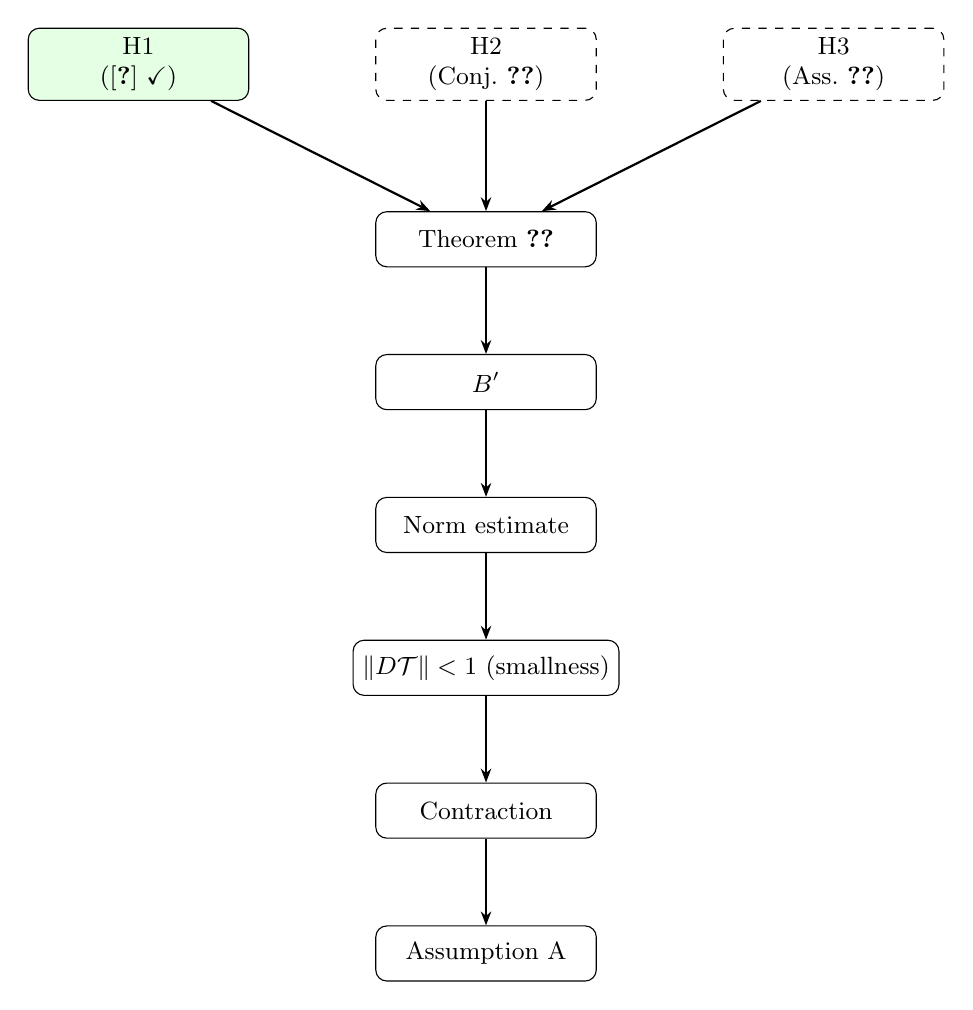
\begin{tikzpicture}[
  node distance=1.1cm and 1.6cm,
  box/.style={draw, rounded corners, minimum width=2.8cm,
              minimum height=0.7cm, align=center, font=\small},
  proved/.style={box, fill=green!10},
  open/.style={box, dashed},
  arr/.style={-{Stealth[length=5pt]}, thick}
]
  \node[proved] (H1)  {H1 \\ (\cite{PhaseNondeg} \checkmark)};
  \node[open, right=of H1] (H2) {H2 \\ (Conj.~\ref{conj:amplitude})};
  \node[open, right=of H2] (H3) {H3 \\ (Ass.~\ref{ass:Bstrong})};

  \node[box, below=1.4cm of H2] (ThmA)
        {Theorem~\ref{thm:dyadic_cancellation}};

  \node[box, below=of ThmA]  (Bp)    {$B'$};
  \node[box, below=of Bp]    (Norm)  {Norm estimate};
  \node[box, below=of Norm]  (Small) {$\|D\mathcal{T}\|<1$ (smallness)};
  \node[box, below=of Small] (Contr) {Contraction};
  \node[box, below=of Contr] (AssA)  {Assumption~A};

  \draw[arr] (H1) -- (ThmA);
  \draw[arr] (H2) -- (ThmA);
  \draw[arr] (H3) -- (ThmA);
  \draw[arr] (ThmA) -- (Bp);
  \draw[arr] (Bp)   -- (Norm);
  \draw[arr] (Norm) -- (Small);
  \draw[arr] (Small)-- (Contr);
  \draw[arr] (Contr)-- (AssA);
\end{tikzpicture}
\end{center}

% ============================================================
% PATCH 3: Open Problems section
% ============================================================
\section{Remaining Open Problems}
\label{sec:open}
% ============================================================

The phase non-degeneracy (Conjecture~6.1 of \cite{paperVI})
is resolved in the companion note \cite{PhaseNondeg}.
The following problems remain open:

\begin{enumerate}[(O1)]
  \item \textbf{ass:gap (uniform Airy spacing in the transition zone):}
    $\lambda_l - \lambda_{l+1} \ge \kappa_0 c^{-1/3}$
    uniformly for $l \le N$.
    This is the next structural target;
    it controls the denominators in B-strong
    and is accessible via the Airy-scale analysis
    of \cite{PhaseNondeg}.

  \item \textbf{B-strong (Assumption~\ref{ass:Bstrong}):}
    $P_{kl} \le C_2 c^{1/2}$ uniformly.
    Depends on ass:gap and Airy amplitude control.

  \item \textbf{Amplitude regularity
    (Conjecture~\ref{conj:amplitude}):}
    $|A_{ij} - A_{i,j+1}| = o(A_{ij}/2^m)$ on dyadic blocks.
    Requires discrete-derivative control of WKB amplitudes,
    addressed in Paper~VIII \cite{paperVIII}.
\end{enumerate}

% ============================================================
\appendix
\section{Complete Proof of Theorem~\ref{thm:dyadic_cancellation}}
\label{sec:appendix}
% ============================================================

We give a complete proof of
Theorem~\ref{thm:dyadic_cancellation}.
Throughout, $i \in \{1,\dots,N\}$ is fixed and all estimates
are uniform in $i$ unless stated otherwise.

\subsection*{Setup}

Recall
\[
  S_m(i) := \sum_{j \in \mathcal{B}_m(i)} T_{ij}
  = \sum_{j \in \mathcal{B}_m(i)}
    \frac{A_{ij}}{|i-j|}\,e^{i\alpha(i-j)}\,e^{i\varepsilon_{ij}}.
\]
We denote by $J_m^- < J_m^+$ the endpoints of the index
range of $\mathcal{B}_m(i)$
(so $J_m^+ - J_m^- \leq 2^{m+1}$),
and write $a_j := A_{ij}$ for the amplitude sequence.

\subsection*{Step 1: Reduction to a Dirichlet sum with error}

On $\mathcal{B}_m(i)$ we have $|i-j| \in [2^m, 2^{m+1})$,
so $|i-j|^{-1} = 2^{-m}(1 + \theta_{ij})$ with
$|\theta_{ij}| \leq 1/2$.
Write $e^{i\varepsilon_{ij}} = 1 + r_{ij}$ where
$|r_{ij}| \leq 2|\varepsilon_{ij}| \leq 2\epsilon_m^{(N)}$
for all $j \in \mathcal{B}_m(i)$ (using $|e^{ix}-1|\leq 2|x|$).
Decompose
\[
  S_m(i)
  = \frac{1}{2^m}
    \underbrace{\sum_{j \in \mathcal{B}_m(i)}
      a_j\,e^{i\alpha(i-j)}}_{=:\,D_m(i)}
  + E_m(i),
\]
where the error satisfies, using $|\mathcal{B}_m(i)|\leq 2^{m+1}$
and (H3),
\[
  |E_m(i)|
  \leq \frac{C}{2^m}\sum_{j\in\mathcal{B}_m(i)}|r_{ij}|
  \leq \frac{C}{2^m} \cdot 2^{m+1} \cdot 2\epsilon_m^{(N)}
  = 4C\,\epsilon_m^{(N)}.
\]
In particular, $|E_m(i)| \leq C'\epsilon_m^{(N)}$
with $C' = 4C$ independent of $m$, $i$, $N$.

\subsection*{Step 2: Abel summation on $D_m(i)$}

Set $b_j := e^{i\alpha(i-j)}$.
Abel summation (summation by parts) gives
\[
  D_m(i)
  = a_{J_m^+} B(J_m^-, J_m^+)
    - \sum_{j=J_m^-}^{J_m^+-1}
      (a_{j+1} - a_j)\, B(J_m^-, j),
\]
where $B(s,t) := \sum_{k=s}^{t} b_k$.

\subsection*{Step 3: Dirichlet kernel bound}

Since $b_j = e^{i\alpha(i-j)}$ is a geometric sequence
with ratio $e^{-i\alpha} \neq 1$
(as $\alpha \not\equiv 0,\pi\pmod{2\pi}$,
now unconditional by Proposition~\ref{prop:H1_nondeg}),
the partial sums satisfy
\[
  \abs{B(s,t)}
  = \left|\frac{e^{i\alpha(i-s)} - e^{i\alpha(i-t-1)}}
               {1-e^{-i\alpha}}\right|
  \leq \frac{2}{\abs{1-e^{i\alpha}}}
  =: C_\alpha < \infty.
\]

\subsection*{Step 4: Total variation estimate}

By hypothesis (H2),
\[
  |a_{j+1} - a_j| \leq \delta_m \frac{a_j}{2^m}
  \leq \delta_m \frac{C}{2^m}.
\]
The block $\mathcal{B}_m(i)$ contains at most $2^{m+1}$
indices, so
\[
  \mathrm{TV}(a;\mathcal{B}_m)
  := \sum_{j=J_m^-}^{J_m^+-1} |a_{j+1}-a_j|
  \leq 2^{m+1} \cdot \delta_m \frac{C}{2^m}
  = 2C\delta_m.
\]

\subsection*{Step 5: Block estimate}

Inserting Steps 3--4 into the Abel decomposition
of Step 2,
\[
  |D_m(i)|
  \leq C_\alpha\,\norm{a}_\infty + C_\alpha\,\mathrm{TV}(a;\mathcal{B}_m)
  \leq C_\alpha C + 2C_\alpha C \delta_m
  =: K(1 + \delta_m),
\]
with $K = C_\alpha C$ independent of $m$, $i$, $N$.
Combining with Step 1,
\[
  |S_m(i)|
  \leq \frac{|D_m(i)|}{2^m} + |E_m(i)|
  \leq \frac{K(1+\delta_m)}{2^m} + C'\epsilon_m^{(N)}.
\]

\subsection*{Step 6: Summation over blocks}

Summing over $m = 0, \dots, M$:
\[
  \sup_i \sum_{j \neq i} |T_{ij}|
  \leq \sum_{m=0}^{M} \sup_i |S_m(i)|
  \leq K \sum_{m=0}^{M} \frac{1+\delta_m}{2^m}
     + C'\sum_{m=0}^{M}\epsilon_m^{(N)}.
\]
The first sum satisfies
$\sum_{m=0}^\infty (1+\delta_m)2^{-m}
\leq 2(1 + \sup_m\delta_m) < \infty$
since $\delta_m \to 0$.
The second sum is $o(1)$ by the summability condition of (H1).
Hence
\[
  \sup_{1\leq i\leq N}\sum_{j\neq i}|T_{ij}|
  \leq 2K + o(1) = O(1). \qed
\]

\begin{remark}[Total phase deviation]
The estimate shows that the total deviation from perfect
cancellation is controlled by
$\sum_m \epsilon_m^{(N)}$,
the sum of block-level phase errors across all dyadic scales.
This quantity measures the \emph{total accumulated phase
deviation} of the kernel from the ideal oscillatory case,
and its vanishing is both necessary and sufficient for
the $O(1)$ row-sum bound to hold.
\end{remark}

% ============================================================
\begin{thebibliography}{9}

\bibitem{paperVI}
[Author],
\textit{No-go theorem for Schur-class estimates of the PSWF
Galerkin operator: layer decomposition and the geometry
of failure},
Paper~VI in this series, preprint 2026.

\bibitem{PhaseNondeg}
[Author],
\textit{Discrete Phase Stability for Prolate Spheroidal Wave
Functions via Airy--WKB Matching},
companion note (\texttt{phase\_nondeg\_lemma.tex}),
prolate-gram-coercivity repository, 2026.

\bibitem{paperVIII}
[Author],
\textit{Scale-Separated Amplitude Estimates for PSWF
Galerkin Operators},
Paper~VIII (skeleton), prolate-gram-coercivity, 2026.

\end{thebibliography}

\end{document}
